\documentclass[UTF8,a4paper,12pt]{ctexart}
\usepackage{geometry}
\usepackage{graphicx}
\usepackage{booktabs}
\usepackage{amsmath}
\usepackage{float}
\usepackage{subcaption}
\usepackage{hyperref}
\usepackage{xcolor}
\usepackage{array}
\usepackage{longtable}
\usepackage{enumitem}

\geometry{left=2.3cm,right=2.3cm,top=2.5cm,bottom=2.5cm}
\graphicspath{{./}{report_images/}}
\hypersetup{colorlinks=true, linkcolor=blue, urlcolor=blue, citecolor=blue}
\setlist[itemize]{leftmargin=2em}
\setlist[enumerate]{leftmargin=2em}

\title{基于 GAN 的人脸图像生成实验报告}
\author{AI2602 深度学习课程项目 · 任务 D}
\date{\today}

\begin{document}
\maketitle

\begin{abstract}
本项目围绕任务 D ``基于 GAN 的人头图像生成'' 展开，目标是在 CelebA 人脸数据集上实现人脸图像生成，并使用 FID 与 Inception Score 对生成质量进行评估。本文首先实现并系统调参了基础 DCGAN 模型，在最佳配置下取得 FID 16.39 的结果；随后在最佳 DCGAN 上进行长时间训练实验，观察到 FID 上升与多样性下降，说明模型存在轻度模式崩溃倾向，并进一步使用 label smoothing 与 instance noise 进行缓解对比。作为改进模型，本文实现了轻量版 StyleGAN-like 结构，引入 mapping network、AdaIN、noise injection 与 R1 regularization，并与 DCGAN 进行对比。最后，本文构造了强制模式崩溃实验，通过破坏生成器与判别器的训练平衡，直观展示 GAN 训练失衡时的生成退化现象。
\end{abstract}

\section{引言}

生成对抗网络（Generative Adversarial Network, GAN）是一类重要的生成模型。它通过生成器（Generator）与判别器（Discriminator）之间的对抗训练，使生成器逐渐学习真实数据分布，从而生成具有真实感的样本。在图像生成任务中，GAN 已经发展出 DCGAN、StyleGAN、CycleGAN 等多种经典结构，其中 DCGAN 是卷积 GAN 的基础代表，StyleGAN 则通过风格控制机制显著提升了高分辨率人脸生成质量。

本项目选择任务 D，即基于 GAN 的人脸图像生成。根据任务要求，基础部分需要实现一个 GAN 模型，完成人脸图像生成、潜变量插值实验，并使用 FID 或 IS 进行评估；Bonus 部分要求对比改进 GAN 模型，并探索 GAN 训练中的模式崩溃问题。本文工作包括：

\begin{itemize}
    \item 实现基础 DCGAN，并在 CelebA 数据集上完成训练、调参与评估；
    \item 对最佳 DCGAN 进行潜变量线性插值实验；
    \item 基于最佳 DCGAN 进行长时间训练，观察自然退化与轻度模式崩溃倾向；
    \item 使用 one-sided label smoothing 与 instance noise 对模式崩溃倾向进行缓解对比；
    \item 实现轻量版 StyleGAN-like 模型，并与基础 DCGAN 进行性能比较；
    \item 构造强制模式崩溃实验，直观展示 GAN 训练失衡时的退化现象。
\end{itemize}

\section{GAN 基本原理}

\subsection{对抗训练思想}

GAN 包含两个神经网络：生成器 $G$ 和判别器 $D$。生成器接收随机噪声 $z \sim p_z$，输出生成样本 $G(z)$；判别器接收真实样本 $x$ 或生成样本 $G(z)$，输出该样本来自真实数据分布的概率。训练过程中，判别器希望正确区分真实样本与生成样本，而生成器希望生成足以欺骗判别器的样本。

标准 GAN 的目标函数可写为：
\begin{equation}
\min_G \max_D V(D,G) =
\mathbb{E}_{x \sim p_{data}(x)}[\log D(x)] +
\mathbb{E}_{z \sim p_z(z)}[\log(1-D(G(z)))] .
\end{equation}

在实际训练中，本项目基础 DCGAN 使用 Binary Cross Entropy Loss。训练判别器时，真实图像标签为 1，生成图像标签为 0；训练生成器时，希望判别器将生成图像判断为真实图像，因此目标标签为 1。

\subsection{评估指标}

本文主要使用 FID 与 Inception Score 评估生成图像质量。

FID（Fr\'{e}chet Inception Distance）通过 Inception 网络特征空间中的均值与协方差，衡量真实图像分布与生成图像分布之间的距离。FID 越低，说明生成分布越接近真实分布。

Inception Score（IS）衡量生成图像的清晰度与类别多样性，通常越高越好。不过本任务是单一人脸领域生成，类别多样性本身有限，因此本文主要依据 FID 与可视化结果进行分析，IS 作为辅助指标。

\section{数据集与实验设置}

\subsection{数据集}

本项目使用 CelebA aligned face images 数据集，共约 202599 张人脸图像。原始数据路径为：
\begin{verbatim}
data/celeba_hf/img_align_celeba/
\end{verbatim}

为了适配 \texttt{torchvision.datasets.ImageFolder} 的目录结构，训练时构造了如下入口：
\begin{verbatim}
data/celeba_imagefolder/
  faces -> data/celeba_hf/img_align_celeba/
\end{verbatim}
GAN 训练不使用类别标签，因此只需一个类别子目录即可。

\subsection{数据预处理与训练环境}

所有图像统一处理为 $64 \times 64$ RGB 图像。预处理包括 resize、center crop、随机水平翻转、转换为 tensor，并归一化到 $[-1,1]$。归一化范围与生成器最后的 \texttt{Tanh} 输出保持一致。

基础训练设置如下：
\begin{itemize}
    \item 图像尺寸：$3 \times 64 \times 64$；
    \item 随机噪声维度：128；
    \item 优化器：Adam；
    \item DCGAN 默认学习率：$2\times 10^{-4}$；
    \item DCGAN 默认 Adam 参数：$\beta_1=0.5,\beta_2=0.999$；
    \item 主要训练硬件：RTX 4090。
\end{itemize}

\section{DCGAN 基础模型}

\subsection{模型结构}

DCGAN 使用卷积结构替代传统全连接网络，生成器通过转置卷积逐步上采样，判别器通过卷积逐步下采样。

生成器输入为随机噪声：
\begin{equation}
    z \in \mathbb{R}^{N \times 128 \times 1 \times 1},
\end{equation}
输出为：
\begin{equation}
    G(z) \in \mathbb{R}^{N \times 3 \times 64 \times 64}.
\end{equation}
生成器主体由 \texttt{ConvTranspose2d + BatchNorm2d + ReLU} 构成，最后一层使用 \texttt{Tanh}。

判别器输入真实图像或生成图像，输出真假概率 $P(real)$。其主体由 \texttt{Conv2d + BatchNorm2d + LeakyReLU} 构成，最后通过 \texttt{Sigmoid} 输出标量概率。判别器结构如图~\ref{fig:dcgan-discriminator} 所示。

\begin{figure}[H]
    \centering
    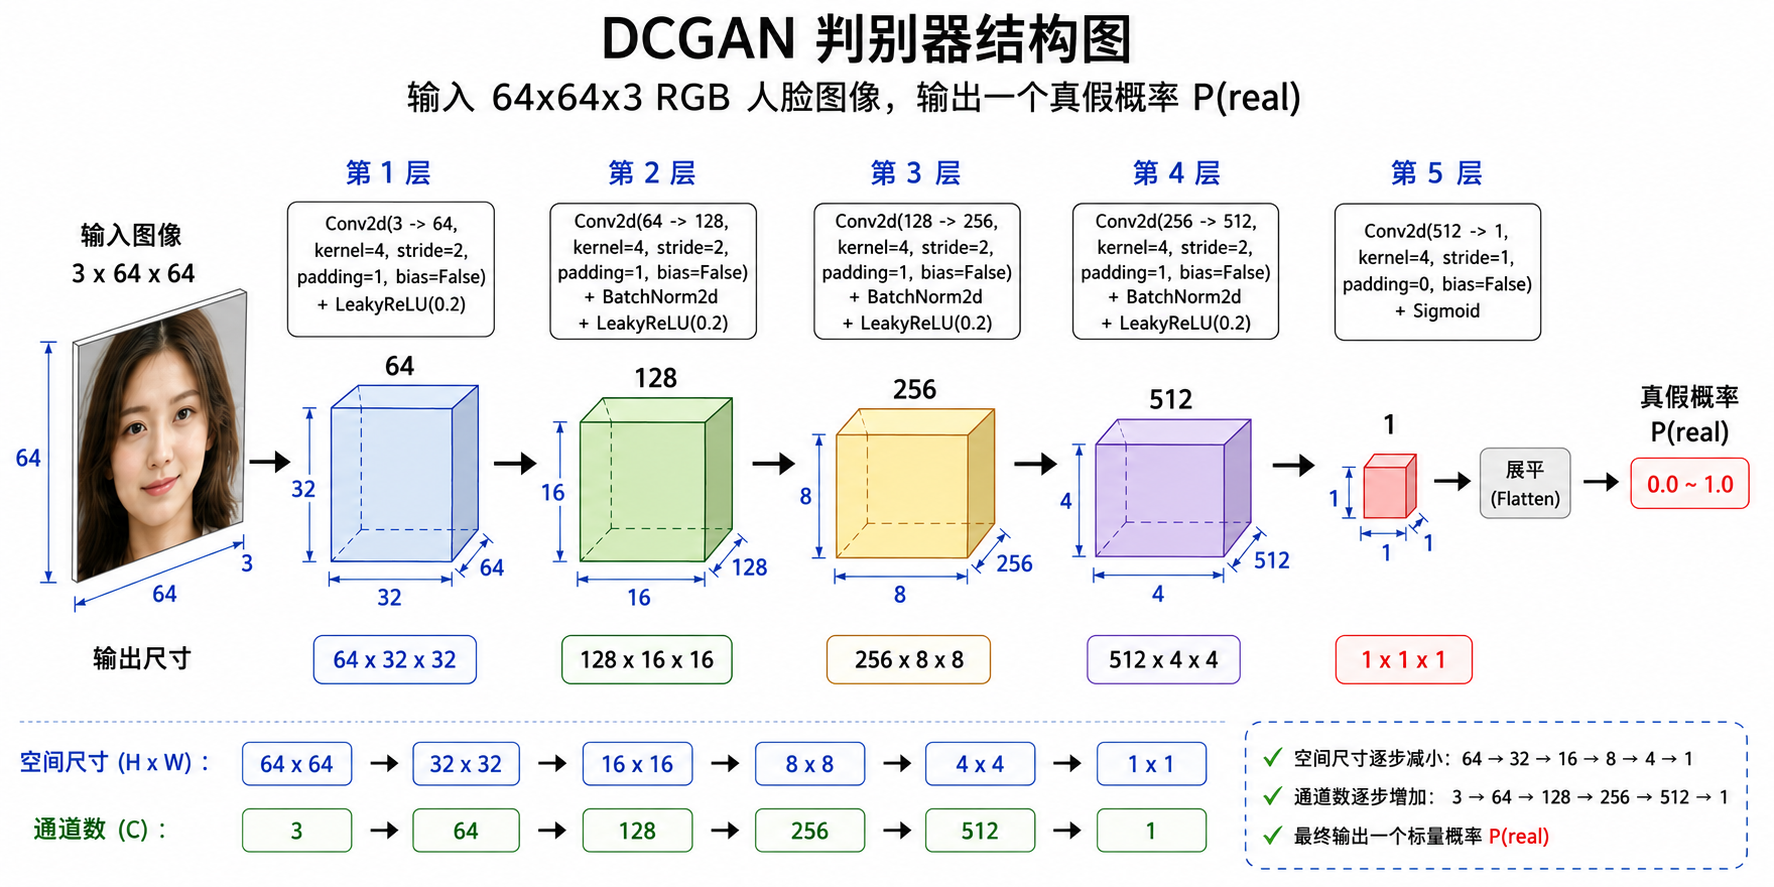
\includegraphics[width=0.98\textwidth]{report_images/dcgan_deciser.png}
    \caption{DCGAN 判别器结构图。输入为 $3\times64\times64$ RGB 人脸图像，输出真假概率 $P(real)$。}
    \label{fig:dcgan-discriminator}
\end{figure}

\section{DCGAN 调参与最终训练}

\subsection{第一轮调参}

为了选择稳定且生成质量较高的配置，首先进行 10 epoch 短轮次调参，并使用 512 张真实/生成图像计算 FID 与 IS。结果如表~\ref{tab:dcgan-tune1} 所示。

\begin{table}[H]
\centering
\caption{DCGAN 第一轮调参结果}
\label{tab:dcgan-tune1}
\resizebox{\textwidth}{!}{%
\begin{tabular}{lrrrrrrrr}
\toprule
实验名称 & Epoch & Batch & LR & $G$通道 & $D$通道 & Eval & FID$\downarrow$ & IS$\uparrow$ \\
\midrule
baseline\_bs128\_lr2e4\_g64\_d64 & 10 & 128 & 0.0002 & 64 & 64 & 512 & 42.970 & 2.152 \\
stable\_bs128\_lr1e4\_g64\_d64 & 10 & 128 & 0.0001 & 64 & 64 & 512 & 41.254 & 2.099 \\
smallbatch\_bs64\_lr2e4\_g64\_d64 & 10 & 64 & 0.0002 & 64 & 64 & 512 & 41.030 & 2.071 \\
largerg\_bs64\_lr2e4\_g128\_d64 & 10 & 64 & 0.0002 & 128 & 64 & 512 & 39.744 & 1.992 \\
\bottomrule
\end{tabular}}
\end{table}

从结果可以看出，减小 batch size 以及增大生成器通道数均有助于降低 FID。第一轮中最优配置为 $batch=64, G=128, D=64$。进一步尝试 $batch=32$ 后，10 epoch FID 降至 33.24，因此最终选择 $batch=32, G=128, D=64$ 作为候选最佳配置。

\begin{figure}[H]
    \centering
    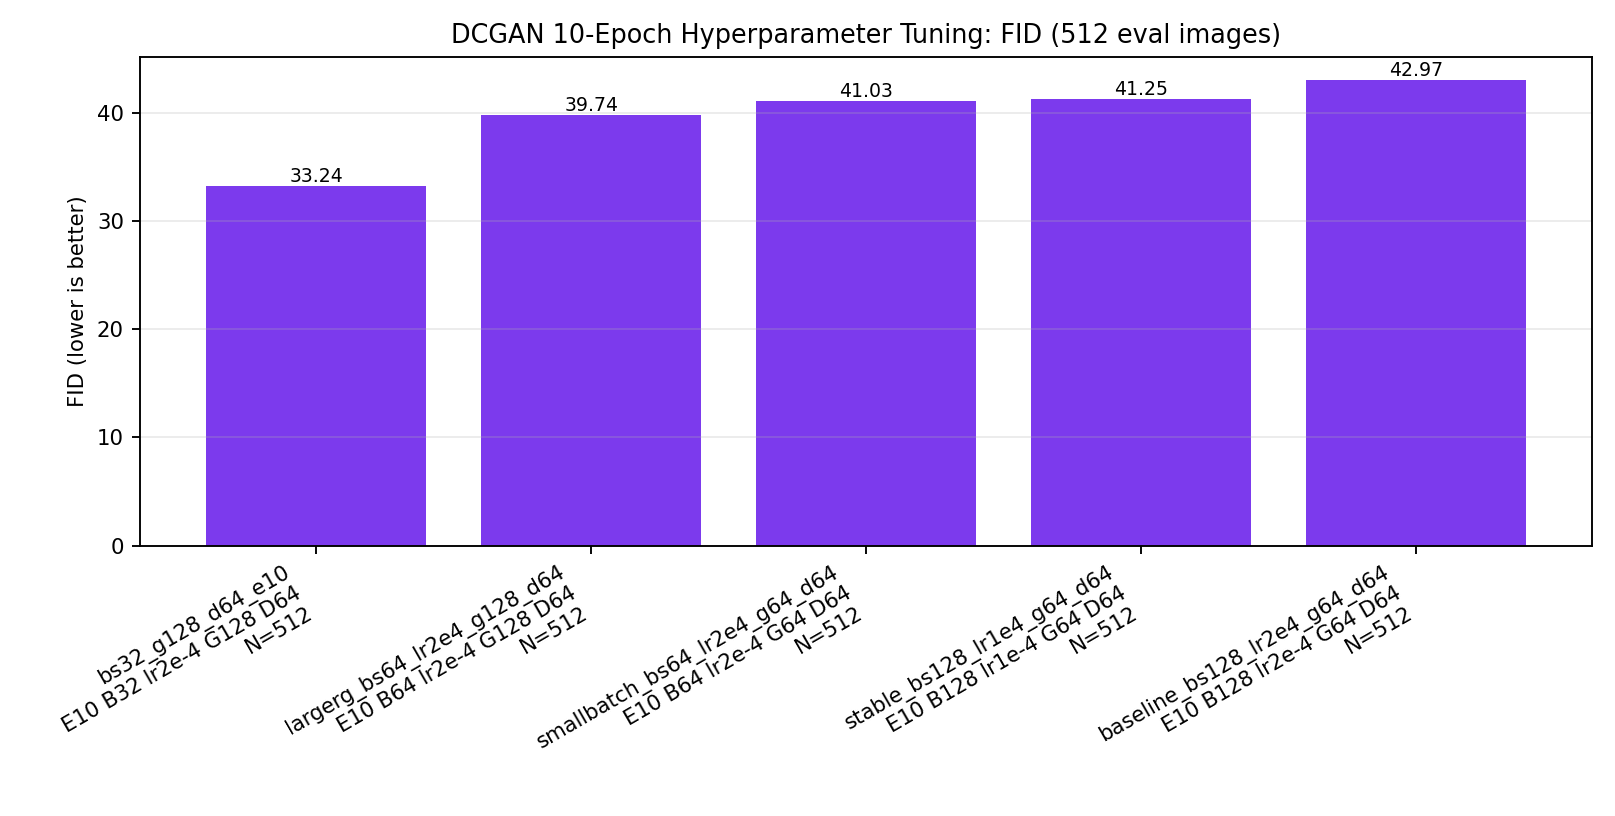
\includegraphics[width=0.72\textwidth]{report_images/dcgan_10epoch_tuning_fid.png}
    \caption{DCGAN 10 epoch 调参 FID 对比。FID 越低表示生成分布越接近真实分布。}
    \label{fig:dcgan-tune-fid}
\end{figure}

\begin{figure}[H]
    \centering
    \begin{subfigure}{0.48\textwidth}
        \centering
        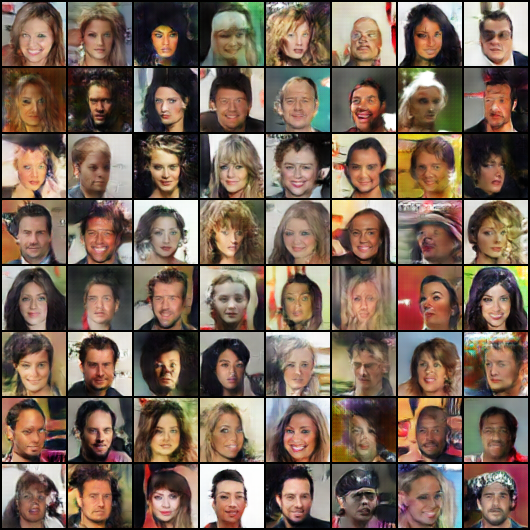
\includegraphics[width=\textwidth]{report_images/tune_baseline_bs128_g64_latest.png}
        \caption{baseline 配置}
    \end{subfigure}
    \begin{subfigure}{0.48\textwidth}
        \centering
        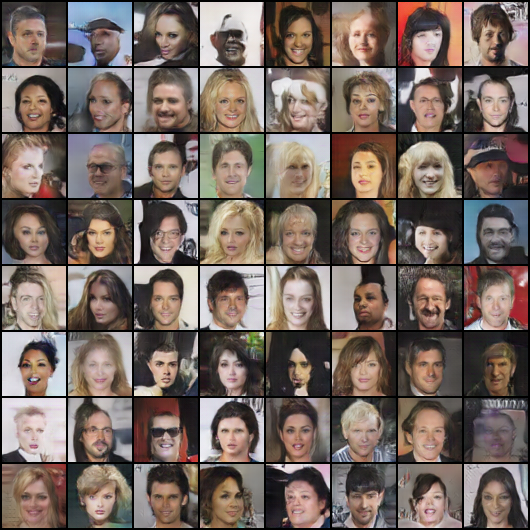
\includegraphics[width=\textwidth]{report_images/tune_largerg_bs64_g128_latest.png}
        \caption{$G=128$ 配置}
    \end{subfigure}
    \caption{DCGAN 不同调参配置下的生成样本。}
\end{figure}

\subsection{最佳参数训练}

最终 DCGAN 采用如下配置：
\begin{equation}
    batch\_size=32, \quad lr=2\times10^{-4}, \quad G=128, \quad D=64.
\end{equation}

该配置在 30 epoch 时 FID 为 19.60，在 50 epoch 时使用 4096 张图像评估，最终 FID 为 16.39，IS 为 2.09。结果如表~\ref{tab:dcgan-final} 所示。

\begin{table}[H]
\centering
\caption{DCGAN 最佳配置不同训练阶段结果}
\label{tab:dcgan-final}
\begin{tabular}{lrrrrr}
\toprule
实验 & Epoch & Eval Images & FID$\downarrow$ & IS$\uparrow$ & IS Std \\
\midrule
bs32\_g128\_d64 & 10 & 512 & 33.243 & 2.046 & 0.104 \\
bs32\_g128\_d64 & 30 & 2048 & 19.603 & 2.192 & 0.125 \\
final\_bs32\_g128\_d64 & 50 & 4096 & 16.394 & 2.093 & 0.071 \\
\bottomrule
\end{tabular}
\end{table}

\begin{figure}[H]
    \centering
    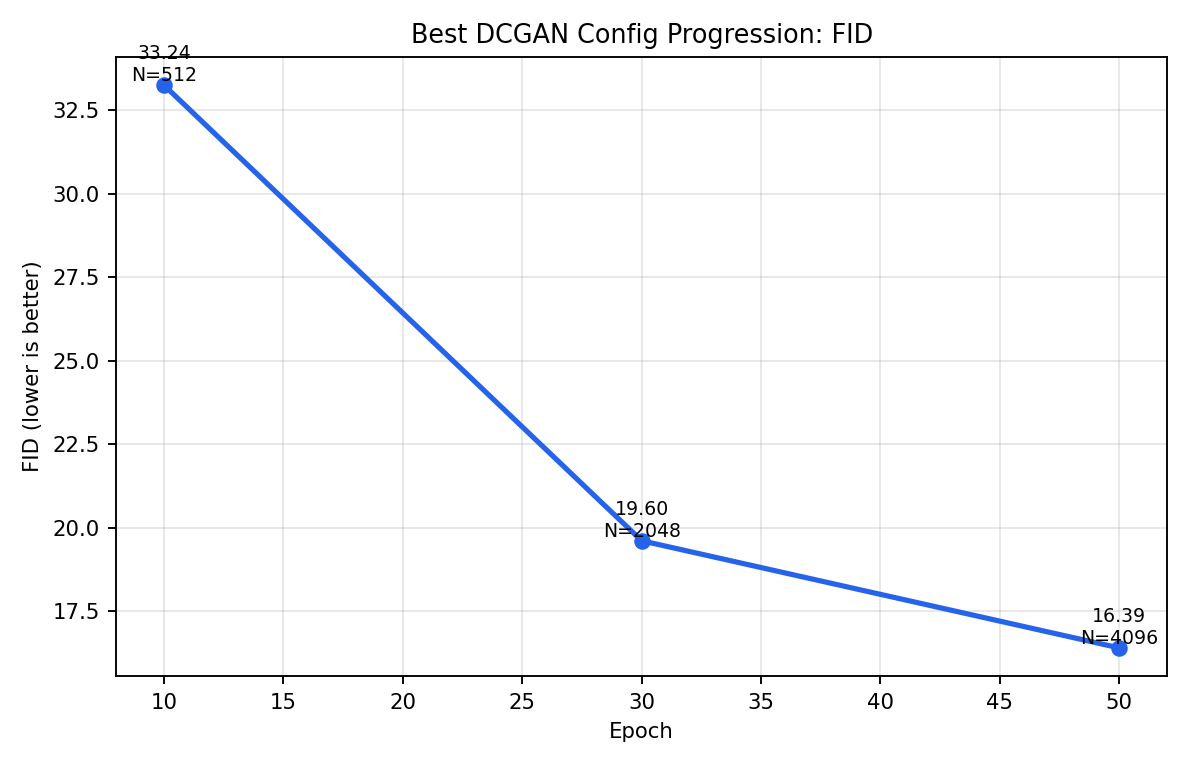
\includegraphics[width=0.72\textwidth]{report_images/dcgan_best_config_fid_progression.png}
    \caption{DCGAN 最佳配置随训练轮次增加的 FID 变化。}
\end{figure}

\begin{figure}[H]
    \centering
    \begin{subfigure}{0.32\textwidth}
        \centering
        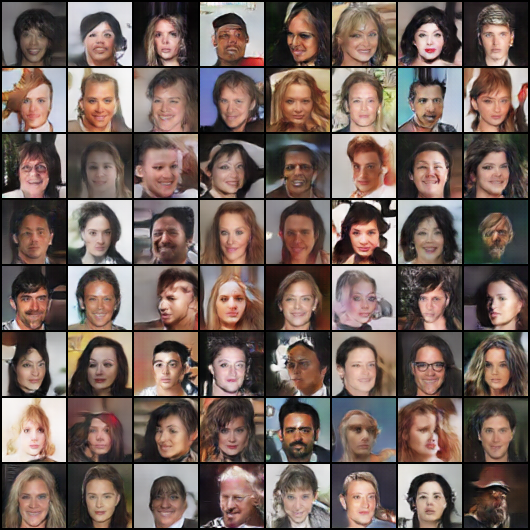
\includegraphics[width=\textwidth]{report_images/final_samples_epoch_0005.png}
        \caption{Epoch 5}
    \end{subfigure}
    \begin{subfigure}{0.32\textwidth}
        \centering
        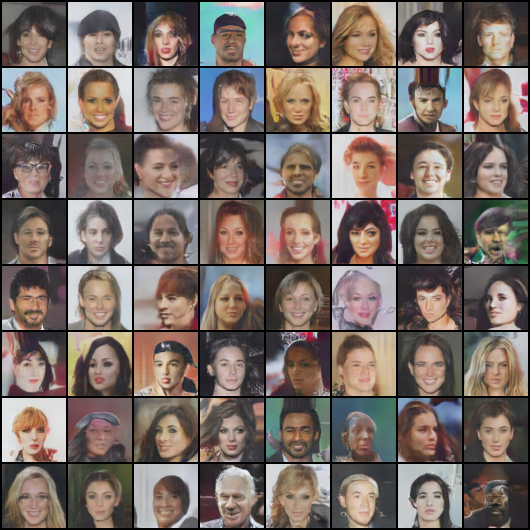
\includegraphics[width=\textwidth]{report_images/final_samples_epoch_0025.png}
        \caption{Epoch 25}
    \end{subfigure}
    \begin{subfigure}{0.32\textwidth}
        \centering
        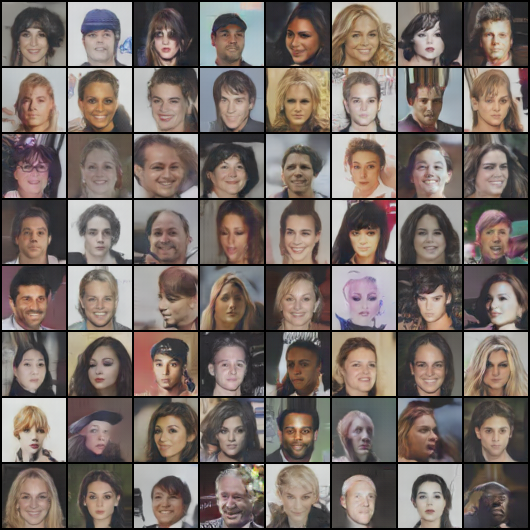
\includegraphics[width=\textwidth]{report_images/final_samples_epoch_0050.png}
        \caption{Epoch 50}
    \end{subfigure}
    \caption{DCGAN 最佳配置训练过程中生成样本的变化。}
\end{figure}

\begin{figure}[H]
    \centering
    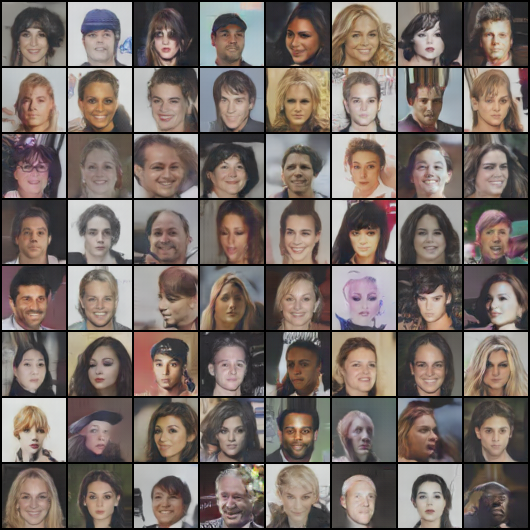
\includegraphics[width=0.66\textwidth]{report_images/final_samples_latest.png}
    \caption{DCGAN 最佳配置最终生成样本。}
    \label{fig:dcgan-final-samples}
\end{figure}

从可视化结果可以看到，训练早期生成图像存在明显噪声和结构不稳定；随着训练进行，人脸轮廓、肤色与五官结构逐渐清晰。最终样本已经能够生成较完整的人脸结构，但在细节一致性和背景稳定性方面仍有提升空间。

\subsection{潜变量线性插值}

为了验证生成器是否学习到了连续的潜变量空间，在两个随机潜变量 $z_1,z_2$ 之间进行线性插值：
\begin{equation}
    z(\alpha) = (1-\alpha)z_1 + \alpha z_2, \quad \alpha \in [0,1].
\end{equation}
插值结果如图~\ref{fig:dcgan-interp} 所示。

\begin{figure}[H]
    \centering
    
\includegraphics[width=0.86\textwidth]{report_images/final_interpolation.png}
    \caption{DCGAN 潜变量线性插值结果。}
    \label{fig:dcgan-interp}
\end{figure}

插值序列中人脸属性呈现相对平滑的变化，说明 DCGAN 学到的潜空间具有一定连续性，而不是仅记忆训练集样本。

\section{最佳 DCGAN 长训与模式崩溃缓解}

\subsection{实验动机}

GAN 训练通常依赖生成器与判别器之间的动态平衡。即使某一配置在中短轮次上表现较好，继续训练也可能导致判别器逐渐占优，生成器分布退化，表现为 FID 上升、多样性下降或模式崩溃倾向。因此本文在最佳 DCGAN 配置上继续训练到 400 epoch，观察长时间训练是否会引发退化。

\subsection{缓解方法}

本文采用两种轻量缓解策略：
\begin{itemize}
    \item \textbf{One-sided label smoothing}：将真实图像标签从 1 改为 0.9，避免判别器过度自信；
    \item \textbf{Instance noise}：在判别器输入的真实图像和生成图像上加入高斯噪声，并随训练线性衰减，降低判别器早期过快压制生成器的风险。
\end{itemize}

对照组均使用同一最佳 DCGAN 配置，差别仅在是否加入上述缓解策略。

\subsection{实验结果}

\begin{table}[H]
\centering
\caption{最佳 DCGAN 长训与缓解策略对比}
\label{tab:natural-collapse}
\resizebox{\textwidth}{!}{%
\begin{tabular}{llrrrrr}
\toprule
组别 & Epoch & FID$\downarrow$ & IS$\uparrow$ & Pixel Div.$\uparrow$ & Pairwise Div.$\uparrow$ & 说明 \\
\midrule
无缓解 & 80 & 21.634 & 2.157 & 0.351 & 0.495 & 长训基线 \\
无缓解 & 160 & 24.442 & 2.196 & 0.313 & 0.445 & FID 上升 \\
无缓解 & 240 & 26.038 & 2.181 & 0.295 & 0.408 & 多样性下降 \\
无缓解 & 320 & 29.864 & 2.185 & 0.299 & 0.413 & 继续退化 \\
无缓解 & 400 & 31.052 & 2.241 & 0.292 & 0.410 & 轻度崩溃倾向 \\
缓解策略 & 80 & 15.232 & 2.268 & 0.551 & 0.768 & 早期明显更好 \\
缓解策略 & 160 & 15.589 & 2.303 & 0.501 & 0.698 & 仍较稳定 \\
缓解策略 & 240 & 30.518 & 2.378 & 0.311 & 0.442 & 后期退化 \\
缓解策略 & 320 & 29.881 & 2.200 & 0.306 & 0.436 & 接近基线 \\
缓解策略 & 400 & 32.030 & 2.206 & 0.292 & 0.419 & 仍未完全解决 \\
\bottomrule
\end{tabular}}
\end{table}

\begin{figure}[H]
    \centering
    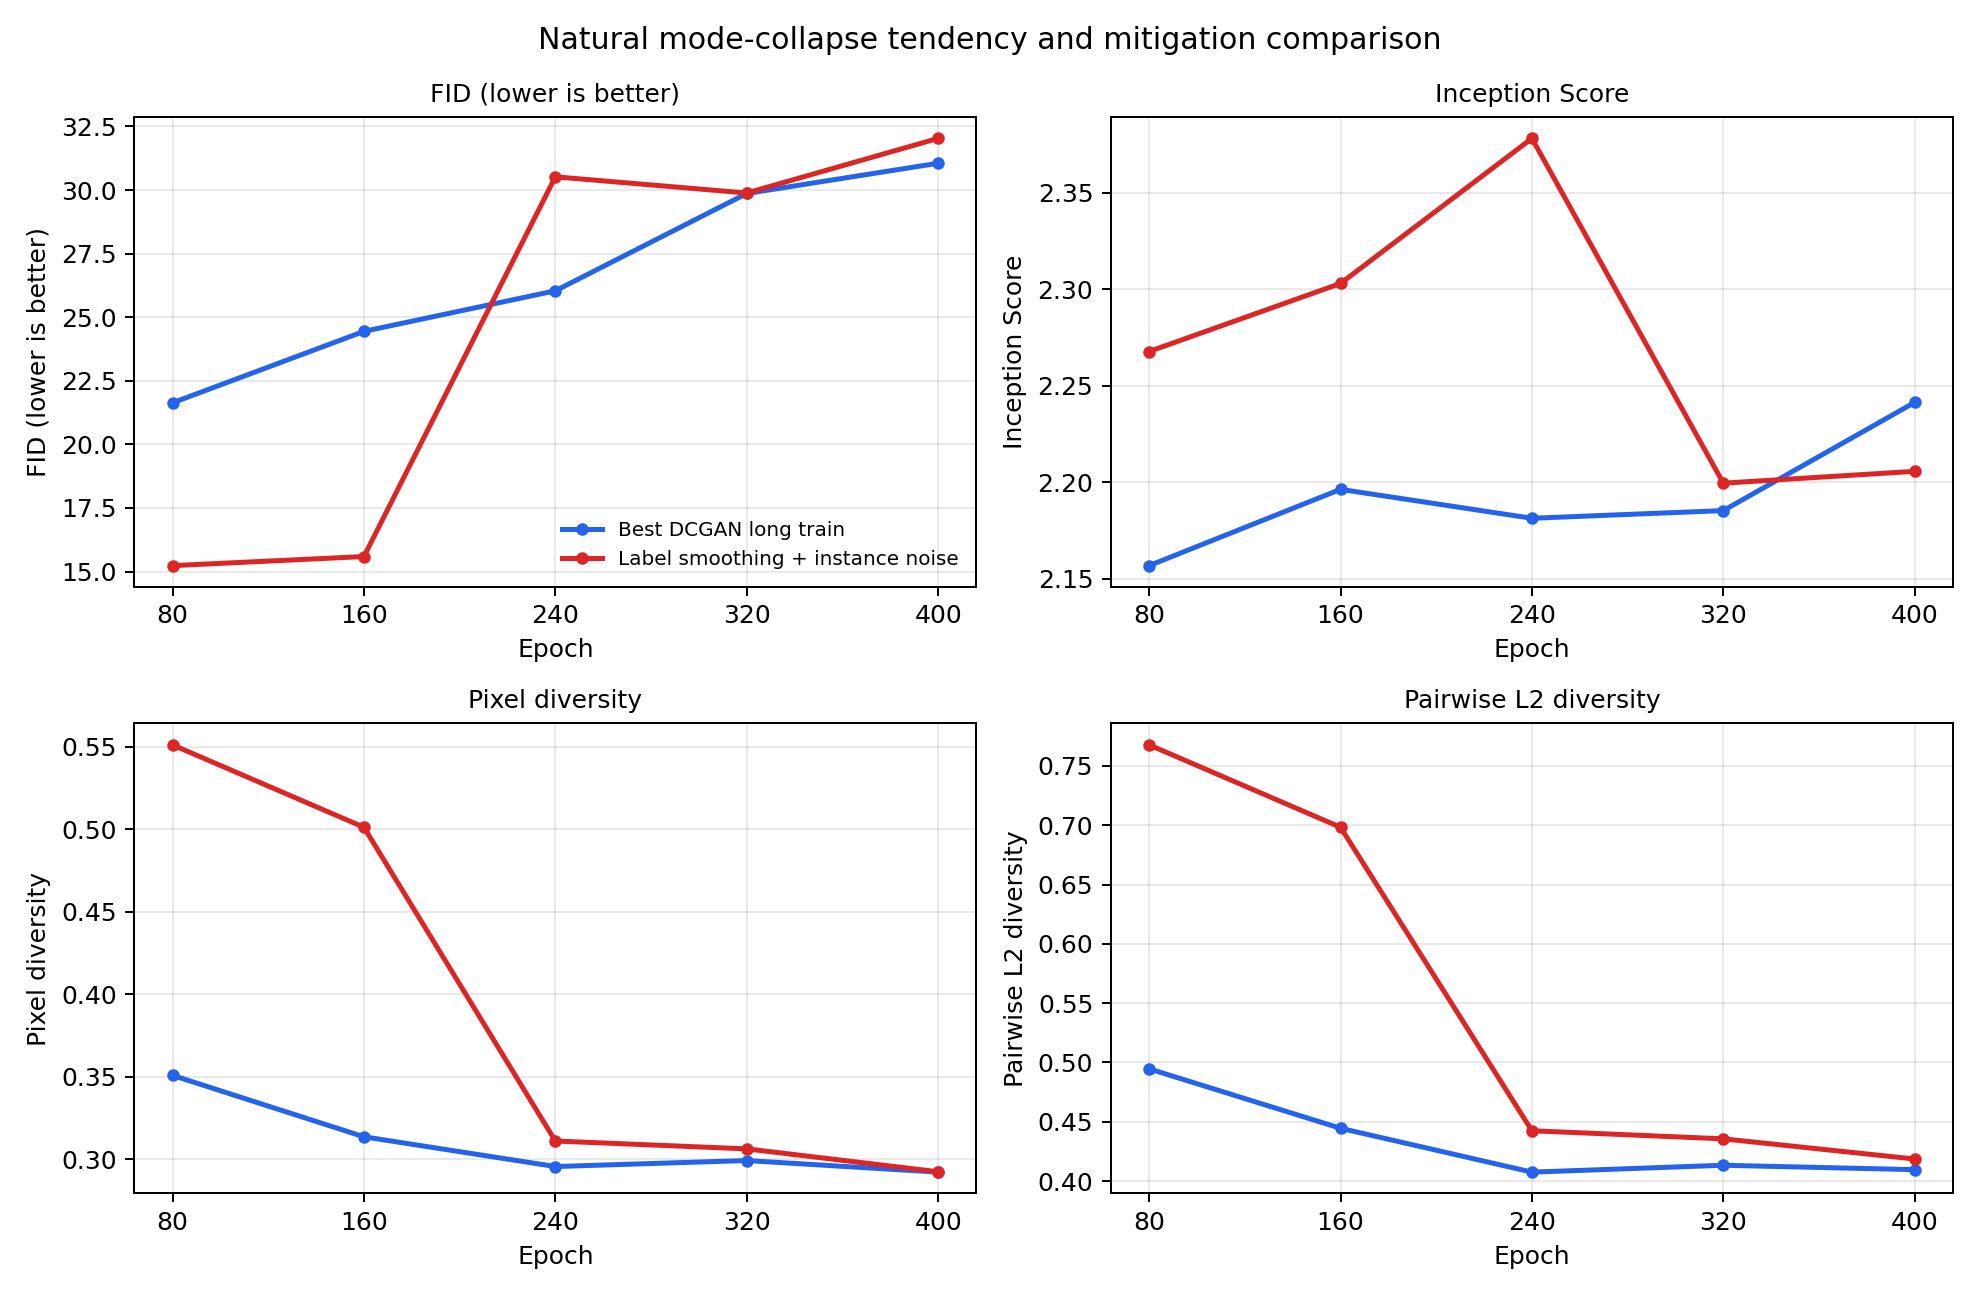
\includegraphics[width=0.92\textwidth]{report_images/mode_collapse_natural_summary_2x2.png}
    \caption{最佳 DCGAN 长训下的 FID、IS 与多样性变化。}
    \label{fig:natural-collapse-summary}
\end{figure}

\begin{figure}[H]
    \centering
    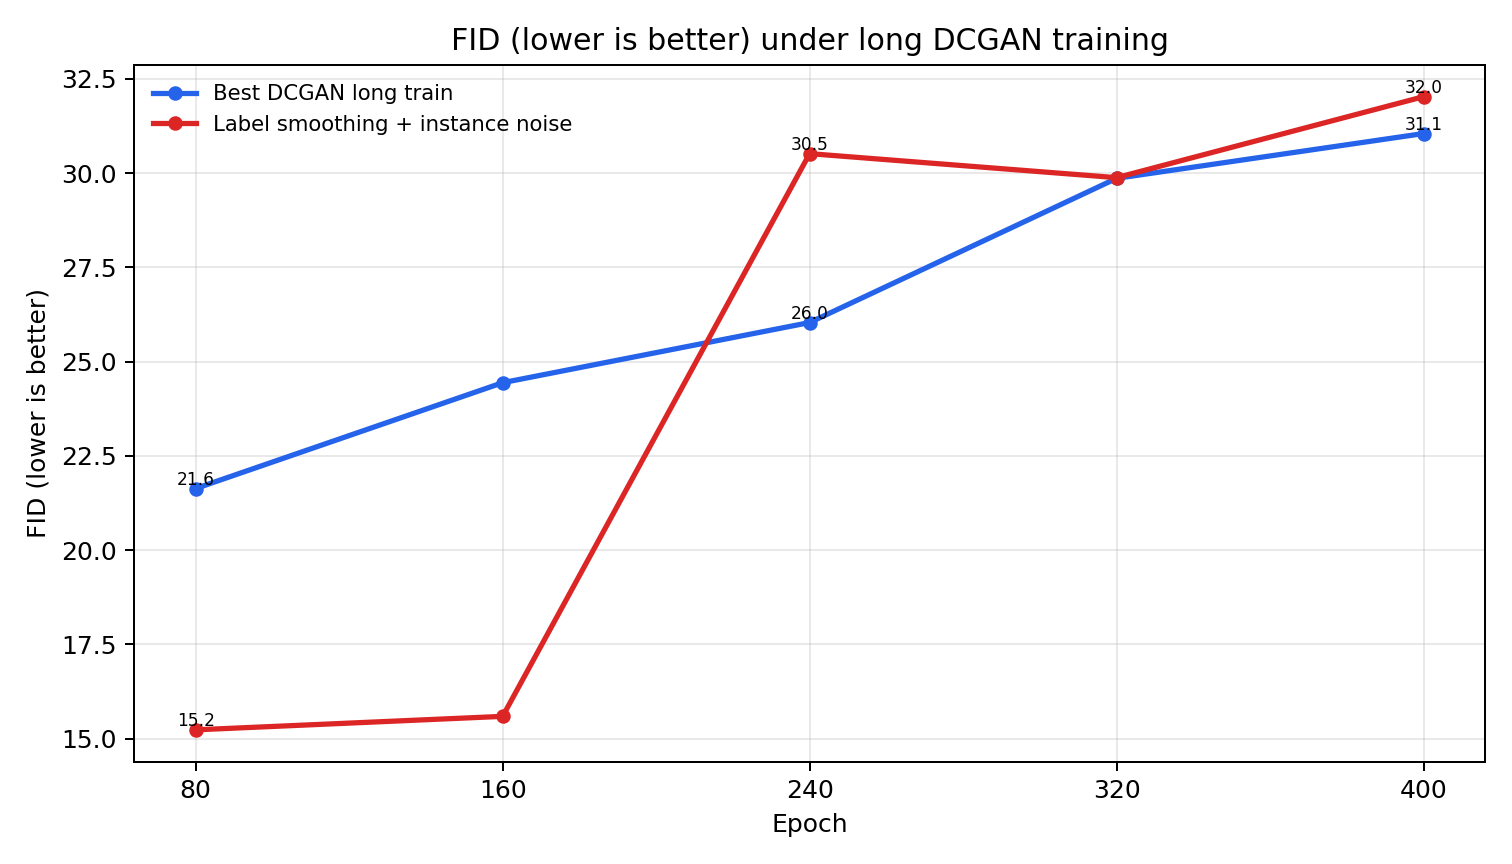
\includegraphics[width=0.72\textwidth]{report_images/mode_collapse_natural_fid.png}
    \caption{长时间训练下 FID 变化。无缓解组 FID 持续升高，说明生成分布逐渐偏离真实分布。}
\end{figure}

无缓解组中，FID 从 80 epoch 的 21.63 上升到 400 epoch 的 31.05，同时 pixel diversity 从 0.351 下降到 0.292，pairwise diversity 从 0.495 下降到 0.410。这说明最佳 DCGAN 在长时间训练下并不是持续改善，而是出现了生成分布退化与轻度模式崩溃倾向。

缓解策略在早期效果明显：80 和 160 epoch 的 FID 分别为 15.23 和 15.59，明显优于无缓解组，同时多样性指标也更高。但 240 epoch 后缓解组也出现退化，说明 label smoothing 与 instance noise 可以延缓早期退化，但不能彻底解决长时间训练下的模式崩溃问题。

需要说明的是，从可视化样本看，长训模型没有完全塌缩为单一图像，因此本文将该现象表述为``轻度模式崩溃倾向''或``生成分布退化''，而非严重模式崩溃。

\section{轻量版 StyleGAN-like 改进模型}

\subsection{模型动机}

DCGAN 直接将随机噪声输入生成器，控制能力较弱。StyleGAN 的核心思想是将随机噪声先映射到中间风格空间，再通过风格调制控制不同层级的图像属性。为了在课程项目规模内探索 StyleGAN 思想，本文实现了轻量版 StyleGAN-like 模型。

\subsection{模型结构}

轻量版 StyleGAN-like 模型包含 mapping network、learned constant、AdaIN、noise injection、ToRGB 与判别器。整体结构如图~\ref{fig:stylegan-like-arch} 所示。

\begin{figure}[H]
    \centering
    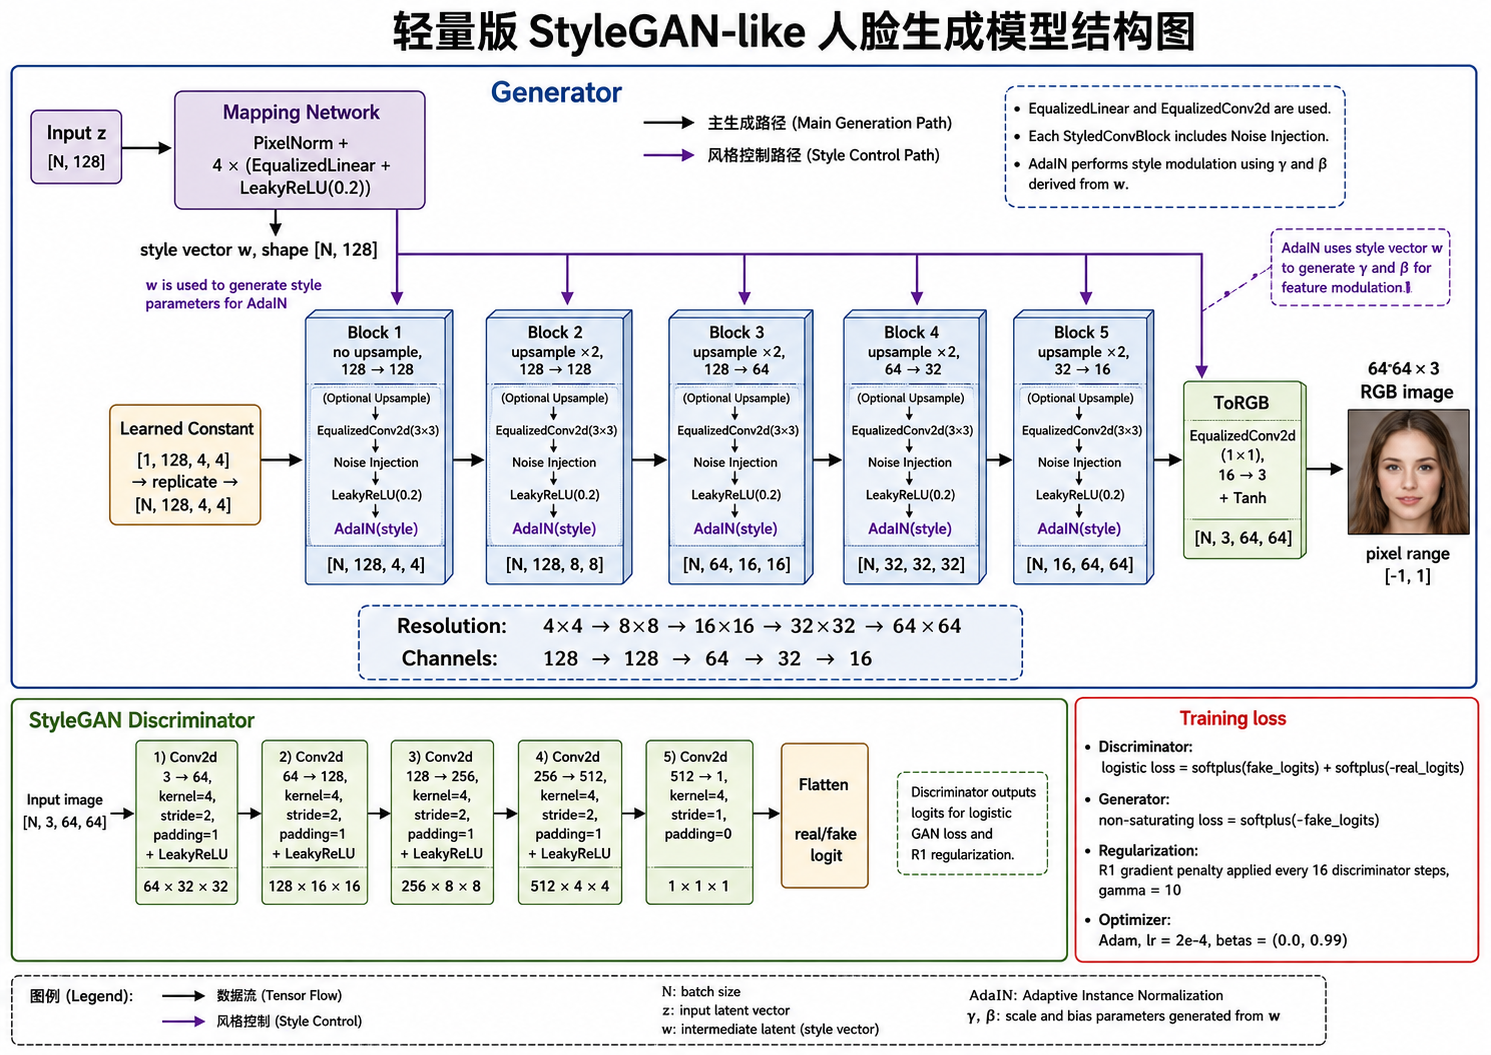
\includegraphics[width=0.98\textwidth]{report_images/stylegan_like.png}
    \caption{轻量版 StyleGAN-like 人脸生成模型结构。}
    \label{fig:stylegan-like-arch}
\end{figure}

该实现并非 NVIDIA 完整原版 StyleGAN，而是面向本项目的轻量实现。主要区别在于：本文没有实现完整 progressive growing、path length regularization 和大规模高分辨率训练，而是保留 StyleGAN 的关键思想，包括 mapping network、style modulation、noise injection 与 R1 regularization。

\subsection{StyleGAN-like 调参}

StyleGAN-like 使用 logistic GAN loss，生成器使用 non-saturating loss，判别器加入 R1 gradient penalty。调参结果如表~\ref{tab:stylegan-tune} 所示。

\begin{table}[H]
\centering
\caption{StyleGAN-like 调参结果}
\label{tab:stylegan-tune}
\resizebox{\textwidth}{!}{%
\begin{tabular}{lrrrrrr}
\toprule
实验名称 & Epoch & Batch & LR & R1 $\gamma$ & FID$\downarrow$ & IS$\uparrow$ \\
\midrule
bs32\_lr2e4\_r1\_10 & 50 & 32 & 0.0002 & 10 & 29.257 & 2.364 \\
bs32\_lr1e4\_r1\_10 & 50 & 32 & 0.0001 & 10 & 45.198 & 2.477 \\
bs64\_lr2e4\_r1\_10 & 50 & 64 & 0.0002 & 10 & 35.587 & 2.410 \\
bs32\_lr2e4\_r1\_5 & 50 & 32 & 0.0002 & 5 & 28.921 & 2.383 \\
\bottomrule
\end{tabular}}
\end{table}

\begin{figure}[H]
    \centering
    \begin{subfigure}{0.48\textwidth}
        \centering
        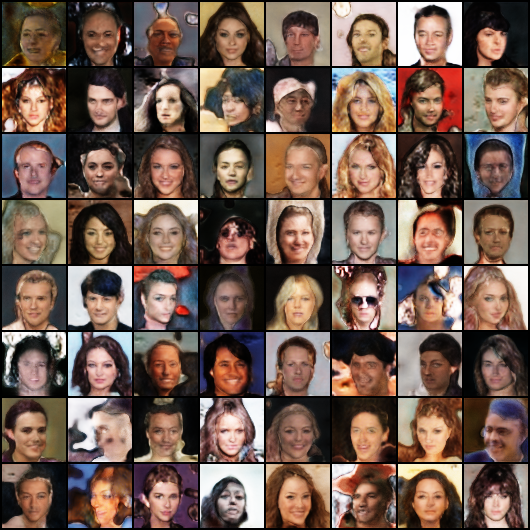
\includegraphics[width=\textwidth]{report_images/stylegan_tune_bs32_lr2e4_r1_10_latest.png}
        \caption{$r1\_\gamma=10$}
    \end{subfigure}
    \begin{subfigure}{0.48\textwidth}
        \centering
        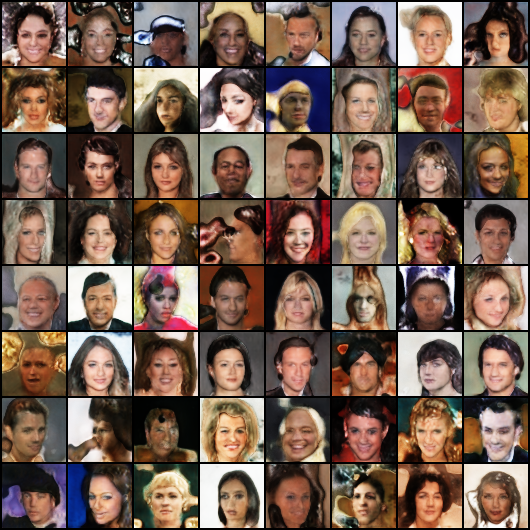
\includegraphics[width=\textwidth]{report_images/stylegan_tune_bs32_lr2e4_r1_5_latest.png}
        \caption{$r1\_\gamma=5$}
    \end{subfigure}
    \caption{StyleGAN-like 不同 R1 配置下的生成样本。}
\end{figure}

调参结果显示，$batch=32, lr=2\times 10^{-4}, r1\_\gamma=5$ 的 FID 最低，因此作为最终训练配置。

\subsection{最终训练与结果分析}

最终 StyleGAN-like 训练 100 epoch，使用 4096 张图像评估，结果为 FID 23.11，IS 2.40。

\begin{table}[H]
\centering
\caption{DCGAN 与 StyleGAN-like 最终结果对比}
\label{tab:dcgan-stylegan-compare}
\begin{tabular}{lrrrr}
\toprule
模型 & Epoch & Eval Images & FID$\downarrow$ & IS$\uparrow$ \\
\midrule
DCGAN & 50 & 4096 & 16.394 & 2.093 \\
StyleGAN-like & 100 & 4096 & 23.114 & 2.400 \\
\bottomrule
\end{tabular}
\end{table}

\begin{figure}[H]
    \centering
    \begin{subfigure}{0.32\textwidth}
        \centering
        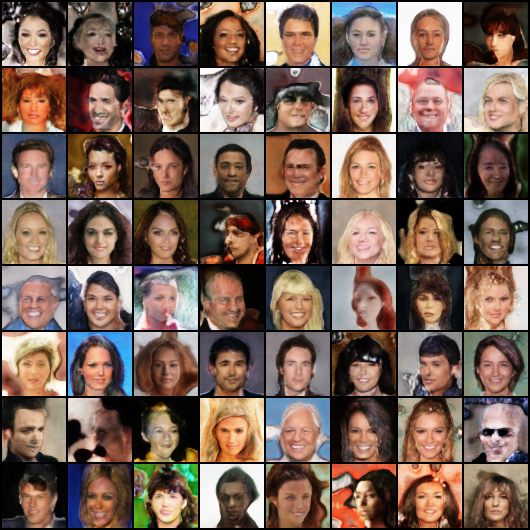
\includegraphics[width=\textwidth]{report_images/stylegan_final_samples_epoch_0050.png}
        \caption{Epoch 50}
    \end{subfigure}
    \begin{subfigure}{0.32\textwidth}
        \centering
        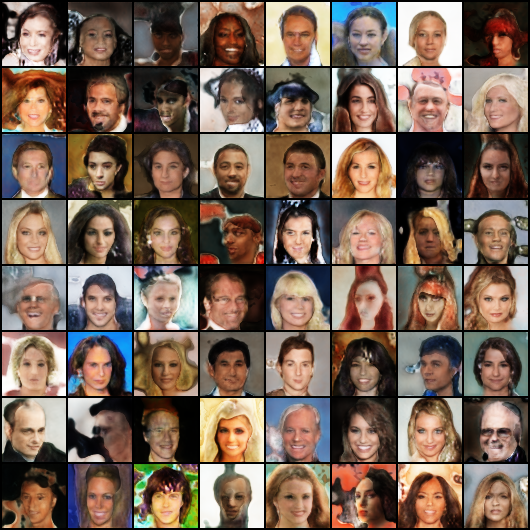
\includegraphics[width=\textwidth]{report_images/stylegan_final_samples_epoch_0100.png}
        \caption{Epoch 100}
    \end{subfigure}
    \begin{subfigure}{0.32\textwidth}
        \centering
        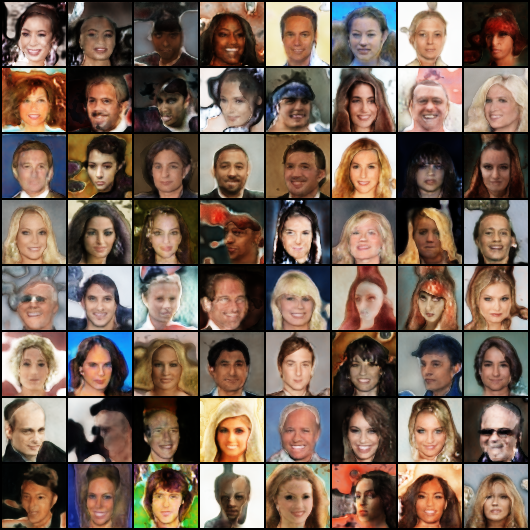
\includegraphics[width=\textwidth]{report_images/stylegan_final_samples_latest.png}
        \caption{Final}
    \end{subfigure}
    \caption{StyleGAN-like 训练过程与最终生成样本。}
\end{figure}

\begin{figure}[H]
    \centering
    
\includegraphics[width=0.82\textwidth]{report_images/stylegan_final_interpolation.png}
    \caption{StyleGAN-like 潜变量插值结果。}
\end{figure}

从 FID 看，轻量版 StyleGAN-like 未超过最终 DCGAN；但从 IS 看，StyleGAN-like 更高，说明其生成样本在 Inception 分类分布上具有更高多样性。考虑到本文实现的是轻量版本，且未采用完整 StyleGAN 的训练策略和更大模型规模，该结果是合理的。StyleGAN-like 的价值主要体现在结构改进和风格控制机制上，而不是在当前资源约束下必然超过 DCGAN。

\section{StyleGAN2 实验预留}

本节预留给 StyleGAN2 实现部分。后续可补充以下内容：
\begin{itemize}
    \item StyleGAN2 相比 StyleGAN 的结构改进；
    \item 实现细节与训练设置；
    \item 生成样本、插值结果与 FID/IS；
    \item 与 DCGAN、StyleGAN-like 的对比分析。
\end{itemize}

\section{强制模式崩溃实验}

\subsection{实验设计}

为了更直观展示 GAN 训练失衡导致的崩溃现象，本文额外构造强制模式崩溃实验。与自然长训实验不同，该实验故意破坏生成器与判别器之间的平衡：

\begin{equation}
noise\_dim=8, \quad G=32, \quad D=128, \quad lr_G=10^{-5}, \quad lr_D=10^{-3}, \quad d\_steps=5.
\end{equation}

该设置显著削弱生成器、增强判别器，并让判别器每轮更新更多次，因此容易导致判别器迅速压制生成器。

\subsection{实验结果}

强制模式崩溃实验训练 10 epoch，评估结果为 FID 336.69，IS 1.0003。IS 接近 1 表明生成图像几乎没有有效多样性，FID 极高说明生成分布严重偏离真实人脸分布。

\begin{figure}[H]
    \centering
    \begin{subfigure}{0.48\textwidth}
        \centering
        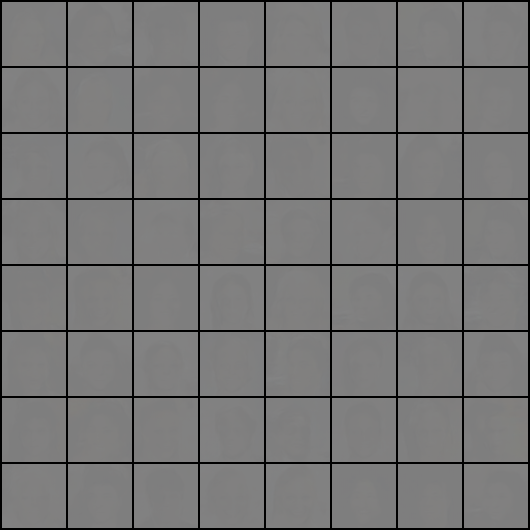
\includegraphics[width=\textwidth]{report_images/mode_collapse_forced_epoch_0007.png}
        \caption{Epoch 7}
    \end{subfigure}
    \begin{subfigure}{0.48\textwidth}
        \centering
        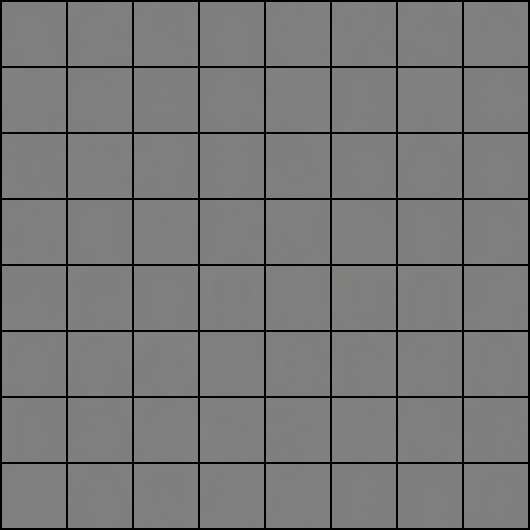
\includegraphics[width=\textwidth]{report_images/mode_collapse_forced_latest.png}
        \caption{Final}
    \end{subfigure}
    \caption{强制模式崩溃实验生成结果。生成图像退化为近似灰色块，缺乏有效人脸结构。}
\end{figure}

该实验说明，GAN 训练对生成器与判别器的相对能力十分敏感。当判别器过强、生成器学习过慢时，生成器无法从判别器中获得有效梯度，最终导致生成样本退化。

\section{综合讨论}

\subsection{实验结果汇总}

\begin{table}[H]
\centering
\caption{主要实验结果汇总}
\label{tab:summary}
\resizebox{\textwidth}{!}{%
\begin{tabular}{lrrrrl}
\toprule
实验 & Epoch & Eval Images & FID$\downarrow$ & IS$\uparrow$ & 说明 \\
\midrule
DCGAN 最佳配置 & 50 & 4096 & 16.394 & 2.093 & 基础模型最终结果 \\
DCGAN 长训无缓解 & 400 & 2048 & 31.052 & 2.241 & 出现轻度退化趋势 \\
DCGAN 缓解组 & 160 & 2048 & 15.589 & 2.303 & 早期缓解有效 \\
DCGAN 缓解组 & 400 & 2048 & 32.030 & 2.206 & 后期仍退化 \\
StyleGAN-like & 100 & 4096 & 23.114 & 2.400 & 改进结构，FID 未超过 DCGAN \\
强制模式崩溃 & 10 & 2048 & 336.690 & 1.000 & 严重训练崩溃 \\
\bottomrule
\end{tabular}}
\end{table}

\subsection{主要观察}

第一，系统调参对 DCGAN 结果影响明显。减小 batch size、增大生成器容量后，FID 逐步下降，最终最佳 DCGAN 取得 FID 16.39。

第二，最佳 DCGAN 在 50 epoch 左右表现较好，但继续训练到 400 epoch 后 FID 明显上升，同时多样性下降。这说明 GAN 训练并非越久越好，长期训练可能导致生成分布退化。

第三，label smoothing 与 instance noise 能够显著改善早期长训表现，但在更长训练后仍无法完全阻止退化。这表明简单稳定化技巧可以延缓模式崩溃倾向，但不能根本解决 GAN 训练不稳定问题。

第四，StyleGAN-like 引入了风格映射、AdaIN 和噪声注入等机制，在结构上比 DCGAN 更灵活；但由于本文采用轻量实现，且未完整复现原版 StyleGAN 的训练策略，其 FID 未超过 DCGAN。该结果说明复杂模型并不必然在有限训练资源下获得更优指标。

第五，强制模式崩溃实验直观展示了训练失衡的后果。当判别器过强、生成器过弱时，生成图像迅速退化，FID 极高、IS 接近 1。

\section{总结}

本文完成了任务 D 的基础要求与 Bonus 探索。基础部分实现了 DCGAN 人脸生成系统，完成了调参、最终训练、潜变量插值与 FID/IS 评估。Bonus 部分实现了轻量版 StyleGAN-like 改进模型，并探索了 GAN 训练中的模式崩溃问题：一方面在最佳 DCGAN 长训中观察到轻度分布退化，另一方面通过强制模式崩溃实验展示了严重训练失衡现象。同时，本文尝试使用 label smoothing 与 instance noise 缓解长训退化，结果表明该方法能够改善早期训练稳定性，但无法彻底解决长时间训练下的退化问题。

总体而言，本项目展示了从基础 GAN 实现、系统调参、改进模型对比到训练稳定性分析的完整实验流程。后续工作可以进一步接入完整 StyleGAN2、使用更高分辨率图像、更大模型和更稳定的正则化策略，以进一步提升人脸生成质量。

\begin{thebibliography}{9}
\bibitem{gan} Goodfellow, I. et al. Generative Adversarial Nets. NeurIPS, 2014.
\bibitem{dcgan} Radford, A., Metz, L., and Chintala, S. Unsupervised Representation Learning with Deep Convolutional Generative Adversarial Networks. ICLR, 2016.
\bibitem{stylegan} Karras, T. et al. A Style-Based Generator Architecture for Generative Adversarial Networks. CVPR, 2019.
\bibitem{cyclegan} Zhu, J.-Y. et al. Unpaired Image-to-Image Translation using Cycle-Consistent Adversarial Networks. ICCV, 2017.
\end{thebibliography}

\end{document}
